\section{同じ総時間での選別}\label{sec:selection}

\subsection{設定}

C3 を調べるため，「CIM で $K$ 個の候補を作り，$m$ 個を選んで SA を 1 回ずつかけ，最良値を取る」という手順を，CIM の生成を含めた同じ総時間で比べた．総時間は $T=K t_{\mathrm{CIM}}+m\,t_{\mathrm{SA}}(B)$ とし，LS・指標・試し打ちを使う方法は，その費用の分だけ最後にかける SA の本数を減らした．比べた方法は次のとおりである．
\begin{description}
  \item[無作為] 候補から無作為に $m$ 個を選ぶ．
  \item[cut 上位] 初期カット値の上位 $m$ 個．
  \item[LS 後 cut 上位（基準）] LS 後のカット値の上位．
  \item[多様性] LS 後のカット値の上位 $2m$ 個から，互いに離れた $m$ 個を貪欲に選ぶ．
  \item[試し打ち] 試し打ちの平均の上位．
  \item[学習] ほかの問題だけで学習したリッジ回帰（指標と初期・LS 後のカット値を問題ごとに標準化）の予測の上位．全指標，局所的な指標のみ，固有ベクトル指標のみの 3 通り．評価する問題のデータは学習に使わない．
  \item[ランダム初期化] CIM を使わず，総時間をすべてランダムな初期解からの SA（$T_0=2.0$）に回す．
\end{description}

評価には \ref{sec:gset} 節の SA の結果（候補 512 個 × 16 回）を使い，候補の集合（$K$ 個の部分集合）と各候補の 1 回分の結果を引き直すモンテカルロ（4000 回）で，最良値の期待値を求めた．ランダム初期化の SA は，同じ実装で 500 掃引を 4096 回，5000 掃引を 512 回実行しておき，必要な本数を非復元で引いた．CIM（$K=512$ 本）と SA（512 本）の時間は，ほかの計算がない状態で 24 スレッドで測り，1 本あたりに直した（付録\ref{app:timing}）．LS・指標・固有ベクトルの時間は 1 スレッドで測り，24 で割って同じ並列度に揃えた．方法ごとに使う処理の時間だけを課した（たとえば「LS 後 cut 上位」には LS を，「学習（固有ベクトル指標）」には LS と固有ベクトルの計算 1 回と内積を課す）．

CIM の出力が 1〜5 状態に集まる G15 と G39 は除き，7 問題で比べた．主条件は $T_0=0.5$，5000 掃引，$K=256$，$m=16$ とし，判定は次の 3 つを問題を単位にした片側 Wilcoxon 符号順位検定と Holm の補正で行うと，実行前に固定した．H4a：学習（全指標）が基準より良い．H4b：試し打ちが基準より良い．H4c：基準がランダム初期化より良い．7 問題では全問題が同じ向きでないと補正後に有意にならないので，問題ごとの差も併せて示す．副条件として，$T_0\in\{0.5,2.0\}$，予算 $\{500,5000\}$ 掃引，$(K,m)\in\{(256,16),(64,4)\}$ の残りの組と，LS・指標・試し打ちの費用を 0 とした場合（選別の効果の上限）も求めた．

\paragraph{実行後の変更.} 最初の実行では，\ref{sec:gset} 節の実行で記録した「指標の計算時間」を全ての指標に一律に課していた．この時間には，どの方法も使わない計算（$g_i=0$ の頂点の連結成分）と固有ベクトルの計算が混ざり，逆に LS の時間は入っていなかった．500 掃引ではこの費用が SA 16 本分を超えて評価が止まった．そこで上記のとおり処理ごとに測り直した．また，500 掃引ではランダム初期化に 650〜1600 本が割り当てられるので，当初用意した 512 本からの復元抽出では最良値を過小に見積もる．4096 本を追加で用意し，非復元抽出に改めた．さらに，\ref{sec:gset} 節の実行は一部がほかの計算と重なっており，同じ seed の CIM の時間が 2 つの開始温度の実行で最大 2.3 倍違った．ランダム初期化に回す本数は CIM と SA の時間の比で決まるので，時間をほかの計算がない状態で測り直した．修正前の 2 つの版（記録した時間による評価）でも，主条件の 3 つの判定の結果は同じだった．

\subsection{結果}

\begin{table}[t]
\centering
\caption{同じ総時間での比較（$K=256$，$m=16$）．BKS との差（\%）の 7 問題の平均．「—」は少なくとも 1 問題で費用が予算を超え，SA を 1 本もかけられないもの．}\label{tab:selection}
\small
\begin{tabular}{lcccc}
\toprule
 & \multicolumn{2}{c}{$T_0=0.5$} & \multicolumn{2}{c}{$T_0=2.0$} \\
方法 & 500 掃引 & 5000 掃引 & 500 掃引 & 5000 掃引 \\
\midrule
無作為 & 0.549 & 0.346 & 0.629 & 0.299 \\
cut 上位 & \textbf{0.431} & 0.265 & \textbf{0.536} & 0.302 \\
LS 後 cut 上位（基準） & \textbf{0.431} & 0.263 & 0.538 & 0.302 \\
多様性 & 0.441 & 0.279 & 0.538 & 0.304 \\
試し打ち & --- & 0.274 & --- & 0.322 \\
学習（全指標） & 0.435 & 0.267 & 0.540 & 0.303 \\
学習（固有ベクトル指標） & 0.432 & 0.265 & 0.540 & 0.302 \\
ランダム初期化 & 0.612 & \textbf{0.221} & 0.610 & \textbf{0.222} \\
\bottomrule
\end{tabular}
\end{table}

\begin{figure}[t]
\centering
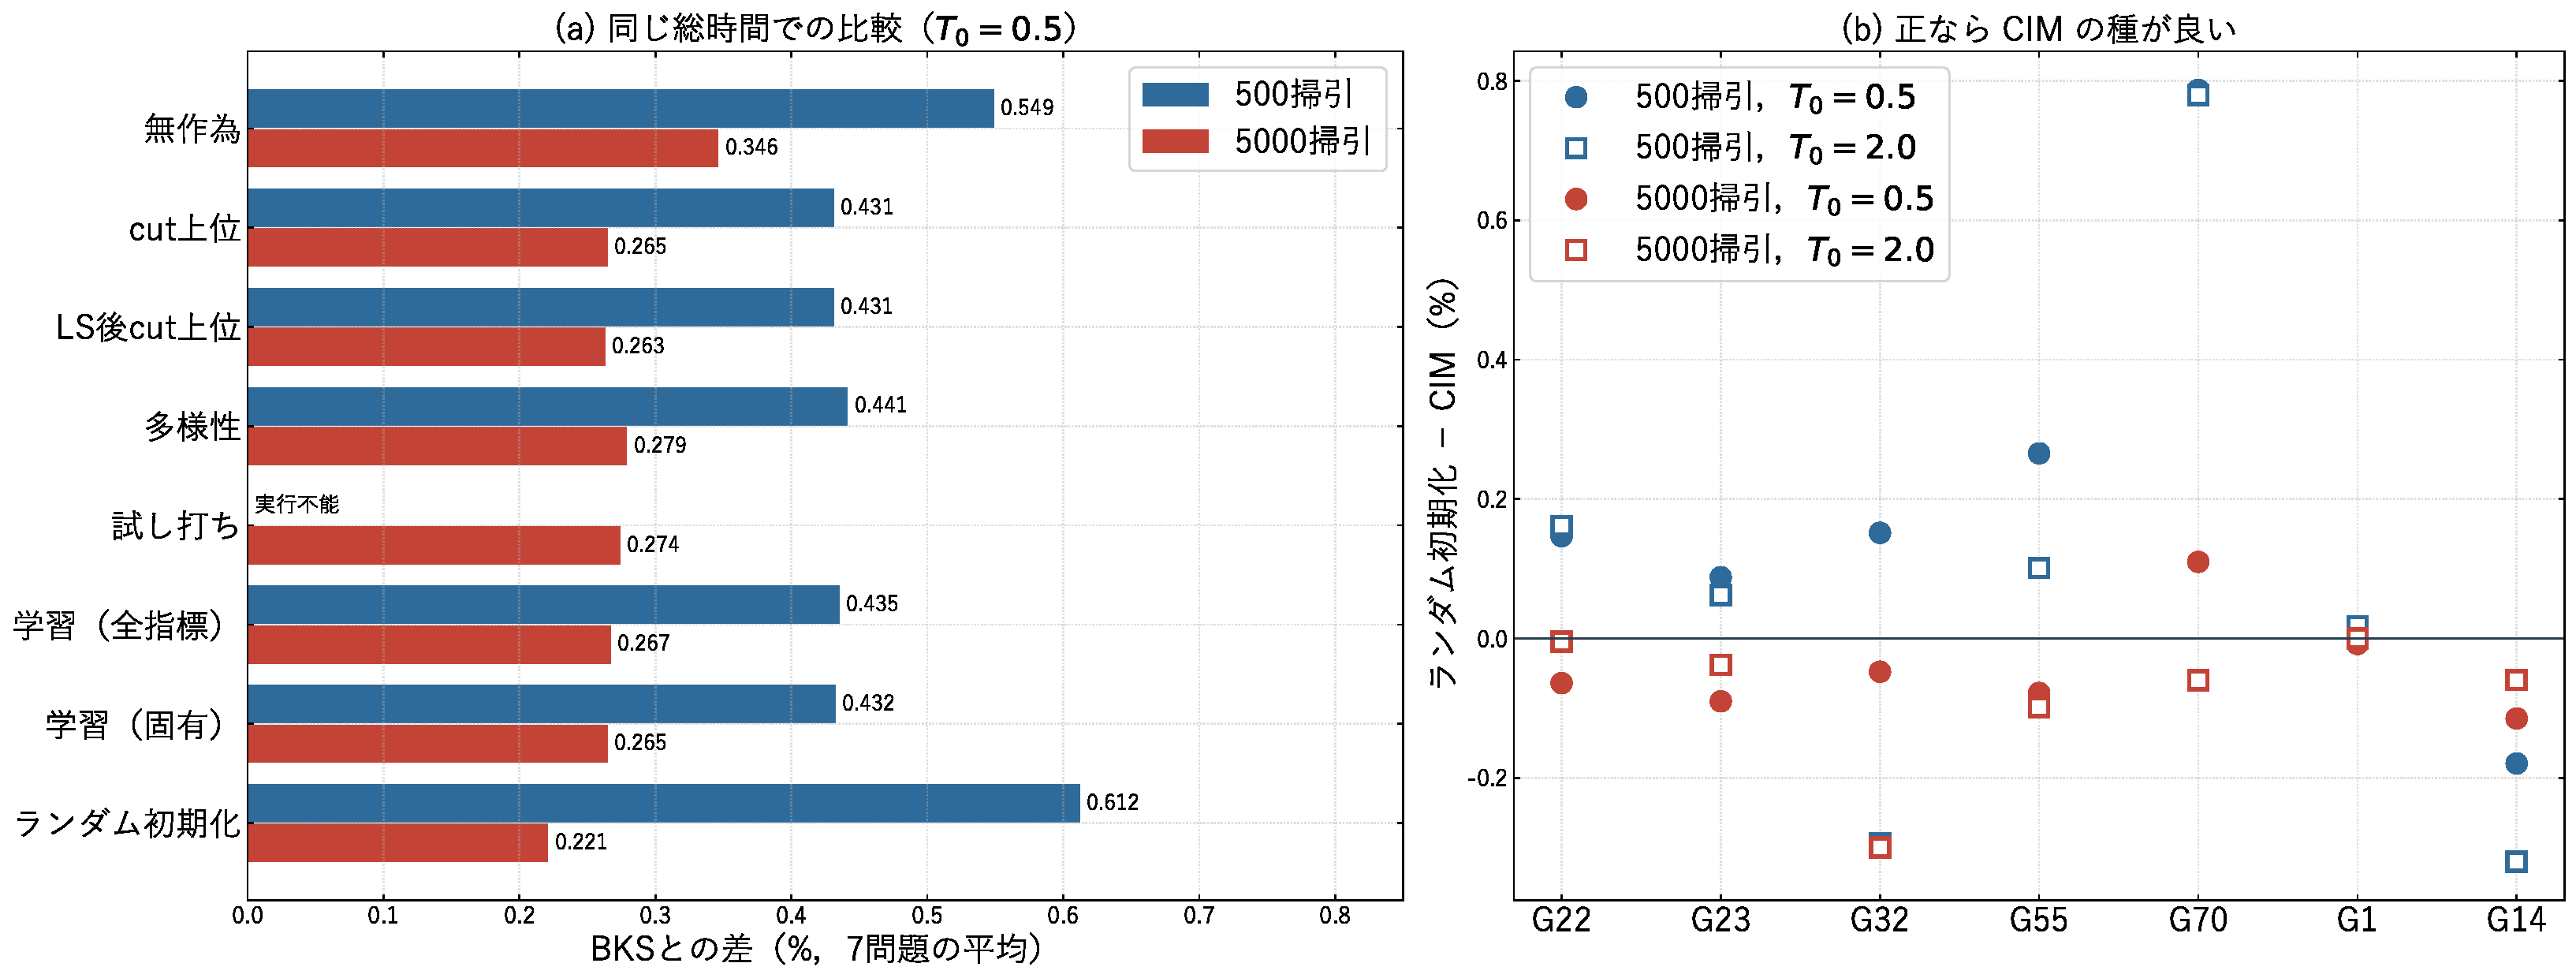
\includegraphics[width=\linewidth]{fig_selection.pdf}
\caption{(a) 主条件（$T_0=0.5$，$K=256$，$m=16$）での各方法の BKS との差．(b) 問題ごとの「ランダム初期化 $-$ LS 後 cut 上位」の BKS との差（正なら CIM の種が良い）．}\label{fig:selection}
\end{figure}

\paragraph{主条件では 3 つの判定がいずれも成り立たなかった.} 学習（全指標）は基準に対して 1 勝 6 敗（片側 $p=0.95$），試し打ちは 0 勝 7 敗（$p=1.00$）であり，基準はランダム初期化に対して 1 勝 6 敗（$p=0.92$）だった（表\ref{tab:selection}，図\ref{fig:selection}）．

\paragraph{カット値を超える選別は役に立たない.} 候補を無作為に選ぶより，カット値で選ぶほうがはるかに良い（主条件で BKS との差 0.346\% から 0.265\%）．しかし，カット値・LS 後のカット値を超える選別が基準を上回った幅は，8 条件のいずれでも，費用を 0 にした場合を含めて最大 0.003\% だった．費用を課すと，学習や試し打ちはむしろ悪くなった．試し打ちは 500 掃引では費用（50 掃引 × 2 回 × 候補数）が SA の予算全体を超え，実行できなかった．$m=4$ では LS の費用で SA が 1 本減るため，LS をしない「cut 上位」のほうが基準より良かった（$T_0=2.0$・5000 掃引で 0.375\% 対 0.394\%）．固有ベクトル指標が強く効く G22 の主条件でも，学習（固有ベクトル指標）の最良値の期待値は基準と変わらなかった（13349.3 対 13349.4）．

\paragraph{CIM の種の利点は予算が短いときに限られる.} CIM の種とランダム初期化の優劣は，後段の予算で逆転した（図\ref{fig:selection}(b)）．500 掃引では，CIM の種（基準）が 7 問題中 6 問題で良かった（$T_0=0.5$ で平均 0.431\% 対 0.612\%，片側 $p=0.039$，Holm 補正なしの副条件）．特に G70 では差が 0.79\% に達した．5000 掃引では逆に，ランダム初期化が 6 問題で良かった（0.263\% 対 0.221\%）．どちらの予算でも例外は 1 問題ずつだった（500 掃引では G14，5000 掃引では G70）．5000 掃引のランダム初期化は CIM の時間も SA に回すので，1 問題あたり 112〜171 本の SA を実行でき，16 本の CIM の種より最良値が伸びた．
